\documentclass[a4paper]{article}
\usepackage[T1]{fontenc}			% pacchetto per \chapter
\usepackage[italian]{babel}
\usepackage[italian]{isodate}  		% formato delle date in italiano
\usepackage{graphicx}				% gestione delle immagini
\usepackage{amsfonts}
\usepackage{booktabs}				% tabelle di qualità superiore
\usepackage{amsmath}				% pacchetto matematica
\usepackage{enumitem}				% gestione delle liste
\usepackage{pifont}					% pacchetto con elenchi carini
\usepackage{listings}				% pacchetto per i codici
\usepackage[x11names]{xcolor}		% pacchetto colori RGB
% Link ipertestuali per l'indice
\usepackage{xcolor}
\usepackage[linkcolor=black, citecolor=blue, urlcolor=cyan]{hyperref}
\hypersetup{
	colorlinks=true
}

\newcommand{\longline}{\noindent\rule{\textwidth}{0.4pt}}

\definecolor{codegreen}{rgb}{0,0.6,0}
\definecolor{codegray}{rgb}{0.5,0.5,0.5}
\definecolor{codepurple}{rgb}{0.58,0,0.82}
\definecolor{backcolour}{rgb}{0.95,0.95,0.92}
\lstdefinestyle{mystyle}{
	backgroundcolor=\color{backcolour},   
	commentstyle=\color{codegreen},
	keywordstyle=\color{magenta},
	numberstyle=\tiny\color{codegray},
	stringstyle=\color{codepurple},
	basicstyle=\ttfamily\footnotesize,
	breakatwhitespace=false,         
	breaklines=true,                 
	captionpos=b,                    
	keepspaces=true,                 
	numbers=left,                    
	numbersep=5pt,                  
	showspaces=false,                
	showstringspaces=false,
	showtabs=false,                  
	tabsize=2
}

\lstset{style=mystyle}

%\usepackage{showframe}				% visualizzazione bordi
%\usepackage{showkeys}				% visualizzazione etichetta

\newcommand{\dquotes}[1]{``#1''}

\begin{document}
	\author{VR443470}
	\title{Programmazione e sicurezza delle reti}
	\date{\printdayoff\today}
	\maketitle
	
	\newpage
	
	% indice
	\tableofcontents
	
	\newpage
	
	\section{Scrittura di applicazioni di rete mediante interfaccia socket}
	
	\subsection{Host, processo e applicazione}
	
	L'\textcolor{Red3}{\textbf{host}} (colui che ospita) è una \textbf{macchina} sempre identificata da un indirizzo IP a cui, opzionalmente, può essere associato un nome Internet.\newline
	
	\noindent
	Il \textcolor{Red3}{\textbf{processo}} è un \textbf{programma in esecuzione} sull'host, il quale trasmette/riceve pacchetti verso/da altri processi su altri host attraverso la rete. Viene identificato tramite un numero di porta nell'intervallo $0$ - $65535$.\newline
	
	\noindent
	Un \textcolor{Red3}{\textbf{applicazione}} è una collaborazione tra un \textbf{insieme di processi} sparsi sulla rete per fare qualcosa di utile per l'utente, per esempio chat, e-mail, ecc.\newline
	
	\noindent
	Alcuni \textcolor{Green4}{\textbf{esempi}}:
	\begin{itemize}
		\item Eseguendo una ricerca su internet:
		\begin{itemize}
			\item Il \emph{web} è l'applicazione;
			\item Mentre i browser (Chrome, Firefox, Edge, Safari) sono il processo di esecuzione;
			\item L'host è il PC, tablet o smartphone su cui viene aperto il browser;
			\item Apache o NGINX è il processo di esecuzione sulla macchina remota, anch'essa identificata come host.
		\end{itemize}
		
		\item Aprendo un'applicazione come Telegram:
		\begin{itemize}
			\item Telegram è l'applicazione;
			\item Il processo di esecuzione è sempre l'app Telegram che è in esecuzione sul dispositivo attualmente in uso (PC, tablet, ecc.) che funge da host;
			\item Il server di Telegram è il processo di esecuzione sulla macchina remota, anch'essa identificata come host.
		\end{itemize}
	\end{itemize}\newpage

	\subsection{Modalità di trasmissione in Internet}
	
	Su Internet la modalità di trasmissione è una sequenza di byte chiamata: pacchetto, Protocol Data Unit (PDU), Datagram. A seconda del livello del protocollo, ci sono nomi diversi.
	
	\longline
	
	\subsubsection{Applicazioni orientate al datagramma (UDP)}
	
	Alcune \textbf{applicazioni sono orientate al datagramma}, quindi \textbf{ogni pacchetto scambiato tra gli host è indipendente dai precedenti e successivi}. Le \textbf{perdite} di pacchetti non vengono tenute in considerazione ed un \textcolor{Green4}{\textbf{esempio}} può essere la \textbf{trasmissione di temperature}: il ricevitore può non tener conto di alcune perdite poiché le informazioni ricevute non sono necessarie per il futuro.
	
	\longline
	
	\subsubsection{Applicazioni orientate alla connessione (TCP)}
	
	Invece, alcune \textbf{applicazioni sono orientate alla connessione}. A differenza delle applicazioni orientate al datagramma, quelle orientate alla connessione devono tener conto delle perdite poiché solitamente le informazioni scambiate sono di dimensioni rilevanti (e.g. un'immagine). Di conseguenza, una perdita provocherebbe una lettura parziale o impossibile da parte del ricevitore.\newline
	
	\noindent
	Il \textbf{socket} si preoccupa di \textbf{numerare i pacchetti appartenenti alla stessa connessione} per rilevare eventuali pacchetti persi e poterli ritrasmettere.\newline
	
	\noindent
	Il sistema operativo introduce all'interno dei pacchetti un numero di sequenza così che possa rilevare eventuali pacchetti persi e ritrasmetterli.
	\begin{itemize}
		\item \textcolor{Green4}{\textbf{Vantaggi:}}
		\begin{itemize}
			\item L'utente scrive/legge su un archivio remoto con la stessa naturalezza di quando scrive/legge su un archivio locale come se la rete in mezzo non ci fosse.
		\end{itemize}
		
		\item \textcolor{Red3}{\textbf{Svantaggi:}}
		\begin{itemize}
			\item Gli host mittente e destinatario eseguono un lavoro più complesso con il sistema operativo;
			\item Ritardo di ritrasmissione nel caso in cui i pacchetti vengano persi.
		\end{itemize}
	\end{itemize}\newpage

	\subsection{Schemi di applicazioni che utilizzano la rete}
	
	Le applicazioni di rete sono insiemi di processi su host diversi che si scambiano messaggi attraverso la rete. \textbf{Esistono degli schemi base che regolano lo scambio di messaggi}:
	\begin{itemize}
		\item Modello client/server;
		\item Modello Publisher/Subscriber (Pub/Sub)
	\end{itemize}

	\longline
	
	\subsubsection{Modello client/server}
	
	Il \textcolor{Red3}{\textbf{modello client/server}} è quello più utilizzato e funziona nel seguente modo (attenzione all'ordine!):
	\begin{enumerate}
		\item Il \emph{client} esegue una \textbf{richiesta} inviando dei dati al \emph{server};
		
		\item Il \emph{server} riceve i dati del \emph{client}, processa i dati e invia la \textbf{risposta} al \emph{client}. Infine, si mette in attesa di altre richieste.
	\end{enumerate}
	I dati inviati dal \emph{client} possono essere delle trasmissioni di dati o delle richieste di dati. In ogni caso, \textbf{il ruolo è determinato dall'ordine dei messaggi e non dal contenuto}. Si noti che il \emph{client} e \emph{server} \textbf{sono processi e \underline{non host}}. Infatti, l'insieme di un client e un server costituisce l'applicazione di rete.\newline
	
	\noindent
	Un \textcolor{Green4}{\textbf{esempio}} di applicazione client/server è il \textbf{sensore di temperatura corporea} che funge da client e invia al server una temperatura. Le risposte del server sono \dquotes{OK} per confermare l'avvenuta ricezione.\newline
	
	\noindent
	Un altro \textcolor{Green4}{\textbf{esempio}} di applicazione client/server è il display che funge da cliente e chiede al server una temperatura. Le risposte del server in questo caso saranno i dati richiesti.
	
	\longline
	
	\subsection{Creazione dell'interfaccia Socket}
	
	Il programma, prima di utilizzare la rete, deve essere in grado di creare un oggetto di tipo \textbf{socket}. Esso è identificato principalmente da tre parametri:
	\begin{itemize}
		\item Indirizzo IP locale;
		
		\item Porta locale, la quale è un intero senza segno di 16 bit (quindi da 0 a 65'535). Nel modello client/server:
		\begin{itemize}
			\item Il \textbf{server} deve decidere esplicitamente il numero di porta affinché i client possano saperlo (da 0 a 1023 le porte sono chiamate \dquotes{porte note} perché sono utilizzate per protocolli famosi come HTTP);
			
			\item Il \textbf{client} può decidere se scegliere il numero di porta esplicitamente oppure delegare la scelta al sistema operativo.
		\end{itemize}

		\item Modalità di trasmissione: UDP o TCP.
	\end{itemize}\newpage
	
	\subsection{Esempi di codice}
	
	\subsubsection{Esecuzione degli esempi}
	
	\begin{enumerate}
		\item Aprire due terminali
		
		\item Compilare il server e successivamente eseguirlo con il comando:
		\begin{lstlisting}[language=C]
			-gcc network.c serverUDP.c -o serverUDP -lpthread\end{lstlisting}
		
		\item Compilare il client e successivamente eseguirlo con il comando:
		\begin{lstlisting}[language=C]
			-gcc network.c clientUDP.c -o clientUDP -lpthread\end{lstlisting}
	\end{enumerate}

	\longline
	
	\subsubsection{Client UDP}\label{client UDP}
	
	Il client UDP ha il seguente codice:
	\lstinputlisting[language=C]{code/clientUDP.c}
	\begin{itemize}
		\item (4-8) dichiarazione delle variabili tra cui la variabile socket;
	
		\item (10) inizializzazione dell'interfaccia socket sulla porta 20'000;
	
		\item (13) invio, tramite UDP, il messaggio \dquotes{Ciao sono il client!} al destinatario avente indirizzo IP \dquotes{127.0.0.1} (\emph{localhost}) e porta 35'000;
	
		\item (14) attesta dell'arrivo della risposta del server;
		
		\item (15-16) scrittura sul terminale della porta, dell'indirizzo del mittente e del messaggio.
	\end{itemize}\newpage
	
	\subsubsection{Server UDP}\label{server UDP}
	
	Il server UDP ha il seguente codice:
	\lstinputlisting[language=C]{code/serverUDP.c}
	\begin{itemize}
		\item (4-8) dichiarazione delle variabili tra cui la variabile socket;
		
		\item (10) inizializzazione dell'interfaccia socket sulla porta 35'000;
		
		\item (12) attesta dell'arrivo di qualche messaggio da parte di qualche client;
		
		\item (13-14) ricezione di un messaggio da parte di un client e stampa sul terminale dell'indirizzo, della porta e del messaggio del mittente;
		
		\item (15) invio della risposta del server al client.
	\end{itemize}\newpage

	\subsubsection{Client\_inc UDP}
	
	Il client UDP (paragrafo~\ref{client UDP}) può essere riscritto nel seguente modo:
	\lstinputlisting[language=C]{code/clientUDP_inc.c}
	\begin{itemize}
		\item (4-8) dichiarazione delle variabili tra cui la variabile socket;
		
		\item (10) inizializzazione dell'interfaccia socket sulla porta 20'000;
		
		\item (11-12) inserimento di un numero intero da parte dell'utente;
		
		\item (13) invio, tramite UDP, del numero inserito dall'utente al destinatario avente indirizzo IP \dquotes{127.0.0.1} (\emph{localhost}) e porta 35'000;
		
		\item (14) attesta dell'arrivo della risposta del server;
		
		\item (15-16) scrittura sul terminale della porta, dell'indirizzo del mittente e del messaggio.
	\end{itemize}\newpage

	\subsubsection{Server\_inc UDP}
	
	Il server UDP (paragrafo~\ref{server UDP}) può essere riscritto nel seguente modo:
	\lstinputlisting[language=C]{code/serverUDP_inc.c}
	\begin{itemize}
		\item (4-8) dichiarazione delle variabili tra cui la variabile socket;
		
		\item (10) inizializzazione dell'interfaccia socket sulla porta 35'000;
		
		\item (12) attesta dell'arrivo di qualche messaggio da parte di qualche client;
		
		\item (13-14) ricezione di un messaggio da parte di un client e stampa sul terminale dell'indirizzo, della porta e del messaggio del mittente;
		
		\item (15) incremento di uno del valore intero ottenuto;
		
		\item (15) invio della risposta del server al client con il valore incrementato.
	\end{itemize}\newpage

	\subsubsection{Client TCP}\label{client TCP}
	
	Il client TCP ha il seguente codice:
	\lstinputlisting[language=C]{code/clientTCP.c}
	\begin{itemize}
		\item (4-5) dichiarazione delle variabili tra cui la variabile \textsf{connection} per gestire la connessione;
		
		\item (7-8) creazione di una connessione TCP con il server utilizzando \emph{localhost} e la porta 35'000. 
		
		\item (9-10) controllo del valore della connessione per verificare se c'è stato un errore. In tal caso, la connessione termina con la stampa dell'errore su terminale;
		
		\item (12-15) in caso di connessione riuscita, il client richiede l'inserimento di un valore intero all'utente;
		
		\item (16-17) invio del valore intero al server;
		
		\item (18) attesa di una risposta da parte del server;
		
		\item (19-20) al momento della ricezione della risposta, il client stampa la risposta del server e chiude la connessione.
	\end{itemize}\newpage
	
	\subsubsection{Server TCP}\label{server TCP}
	
	Il server TCP ha il seguente codice:
	\lstinputlisting[language=C]{code/serverTCP.c}
	\begin{itemize}
		\item (4-6) dichiarazione delle variabili tra cui la variabile \textsf{connection} per gestire la connessione e \textsf{socket} per gestire i dati;
		
		\item (8) inizializzazione di un socket TCP utilizzando la porta 35'000.
		
		\item (9-10) controllo del valore del socket per verificare se c'è stato un errore. In tal caso, la creazione termina con la stampa dell'errore su terminale;
		
		\item (12-14) in caso di creazione del socket riuscita, il server attende la connessione da parte di qualche client;
		
		\item (15-17) attesa di una richiesta da parte di qualche client. Nel momento in cui viene ricevuta una richiesta, il server la accetta e instaura la connessione e attende la ricezione dei dati;
		
		\item (18-19) all'arrivo dei dati da parte del client, il server esegue un incremento di uno del valore ricevuto dal client;
		
		\item (20-22) il server invia il valore al client e infine chiude la connessione.
	\end{itemize}\newpage

	\subsubsection{Codice per la copia di un file}
	
	Il codice per la copia di un file è strutturato nel seguente modo:
	\lstinputlisting[language=C]{code/fileCopy.c}
	\begin{itemize}
		\item (6-29) dichiarazione dei puntatori ai file e tentativi di apertura dei due file richiesti dall'utente;
		
		\item (32-37) viene eseguita la lettura dal primo file e salvata nella variabile \textsf{c}. A questo punto, finché viene letto un carattere valido, ovvero che non sia la fine del file (\emph{End Of File}, EOF), il contenuto della variabile \textsf{c} viene inserito nel secondo file;

		\item (39-43) al termine del processo di copia, viene stampato il file nel quale sono stati copiati i valori e chiusi i rispettivi file descriptors.
	\end{itemize}\newpage

	\section{Dal Web ai Webservices}
	
	\subsection{Protocollo HTTP/HTTPS}
	
	Il \textcolor{Red3}{\textbf{protocollo HTTP}} venne inventato per fruire dei contenuti in rete (\emph{World Wide Web}). Tuttavia, al giorno d'oggi viene usato per l'invocazione di funzionalità remote, tecnica chiamata \textbf{Webservice}.\newline
	
	\noindent
	Il protocollo si divide in più \textbf{fasi}:
	\begin{enumerate}
		\item Apertura di una connessione TCP;
		
		\item Nel caso del protocollo HTTPS, avviene l'autenticazione del server e negoziazione di una chiave di cifratura;
		
		\item Invio di messaggi di \emph{request} e \emph{response};
		
		\item Chiusura della connessione TCP.
	\end{enumerate}
	\begin{figure}[!htp]
		\centering
		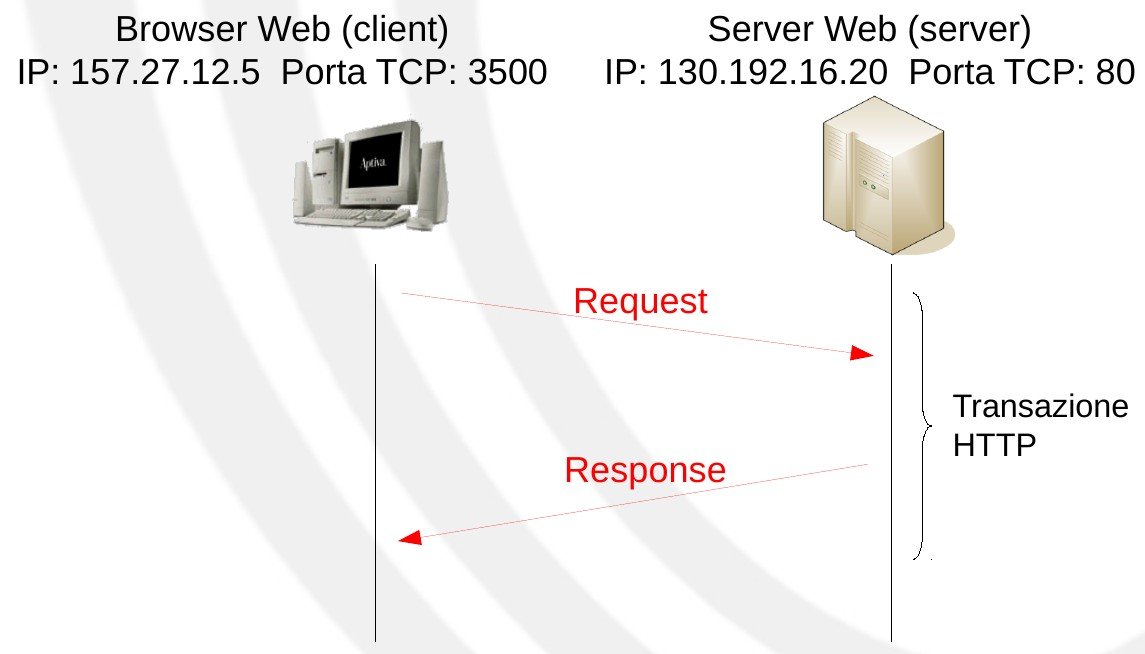
\includegraphics[width=\textwidth]{img/protocollo_http-https.png}
		\caption{Esempio di scambio di messaggi nel protocollo HTTP.}
	\end{figure}\newpage
	
	\noindent
	Nel \textcolor{Red3}{\textbf{protocollo HTTPS}} i messaggi che passano nella connessione TCP, sono gli stessi del protocollo HTTP con l'aggiunta di una \textbf{cifratura dei dati in transito} e di una \textbf{autenticazione del server mediante certificato digitale}. Inoltre, il server lavora sulla porta 443 e non sulla porta classica 80.
	\begin{figure}[!htp]
		\centering
		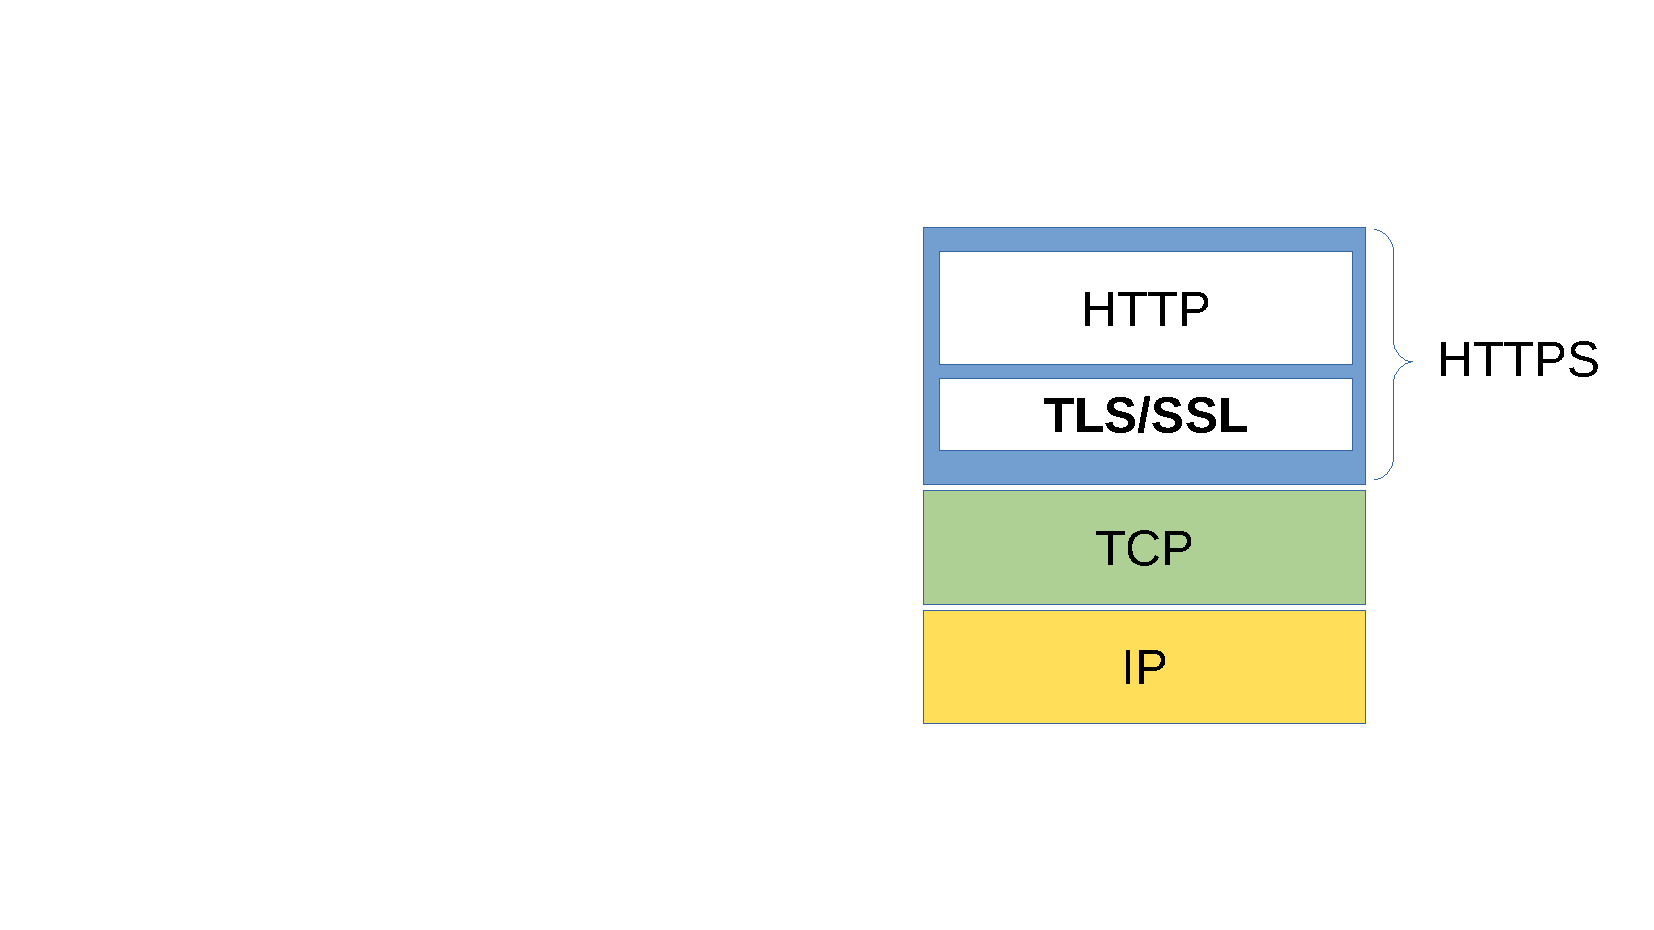
\includegraphics[width=.4\textwidth]{img/protocollo_https.pdf}
		\caption{Protocollo HTTPS.}
	\end{figure}

	\noindent
	Un \textcolor{Green4}{\textbf{esempio}} di richiesta:
	\begin{figure}[!htp]
		\centering
		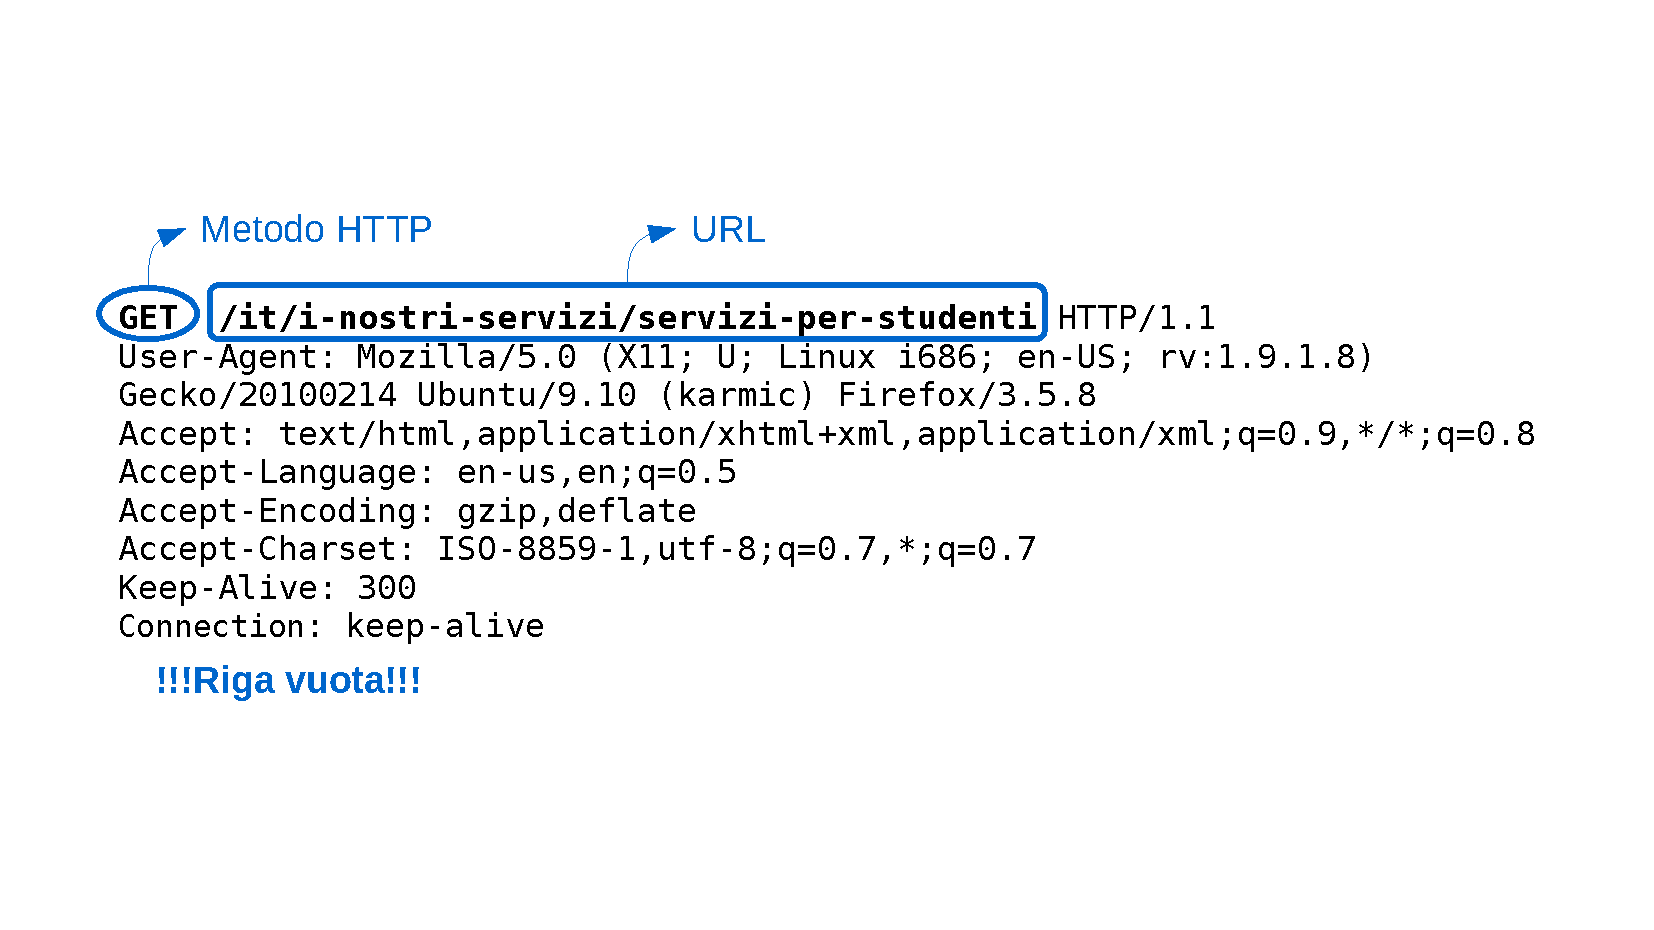
\includegraphics[width=\textwidth]{img/richiesta_http.pdf}
		\caption{Messaggio di richiesta.}
	\end{figure}

	\noindent
	Un \textcolor{Green4}{\textbf{esempio}} di risposta:
	\begin{figure}[!htp]
		\centering
		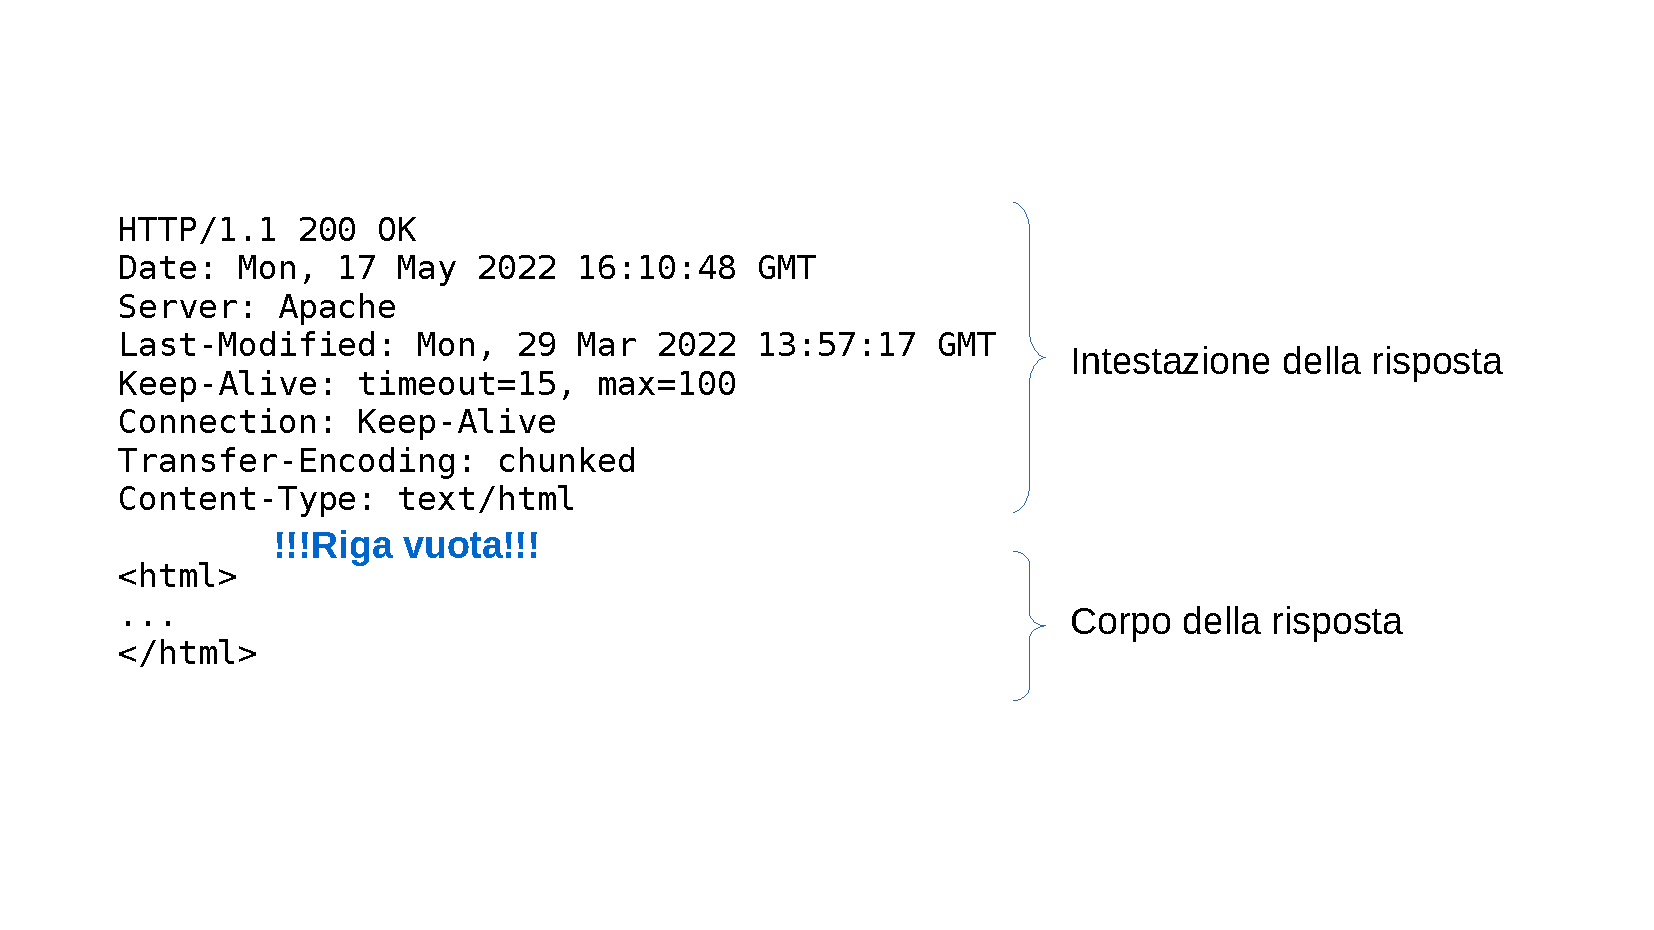
\includegraphics[width=\textwidth]{img/risposta_http.pdf}
		\caption{Messaggio di risposta.}
	\end{figure}\newpage

	\subsection{Hyper Text Markup Language (HTML) e Cascading Style Sheets (CSS)}
	
	\textcolor{Red3}{\textbf{HTML}} è un linguaggio testuale di descrizione di una pagina, in particolare è la specializzazione del generico XML (\emph{eXtensible Markup Language}). HTML si basa sui \dquotes{tag} annidati, i quali eventualmente contengono attributi.\newline
	
	\noindent
	Questo linguaggio, spesso viene utilizzato con un altro linguaggio chiamato \textbf{CSS}.\newline
	
	\noindent
	\textcolor{Green4}{\textbf{Esempi}} di codice HTML:
	\lstinputlisting[language=HTML]{code/css.html}
	E CSS:
	\lstinputlisting{code/styles.css}
	
	\longline
	
	\subsubsection{HTML: tag per richiamare immagini}
	
	Viene utilizzato \dquotes{\textsf{img src}} per richiamare le immagini:
	\lstinputlisting[language=HTML]{code/immagini.html}\newpage
	
	\subsubsection{HTML: tag per il collegamento ipertestuale}
	
	Viene utilizzato \dquotes{\textsf{href}} per il collegamento ipertestuale:
	\lstinputlisting[language=HTML]{code/link.html}
	
	\longline
	
	\subsubsection{Document Object Model (DOM)}
	
	Il \textcolor{Red3}{\textbf{Document Object Model (DOM)}} è una forma di rappresentazione dei documenti (pagina) strutturati come modello orientato agli oggetti.
	
	\longline
	
	\subsection{Javascript}
	
	\textcolor{Red3}{\textbf{Javascript}} è un linguaggio di programmazione multi paradigma orientato agli eventi, utilizzato sia nella programmazione lato client web che lato server. È facile trovarlo all'interno di codice HTML anche grazie al suo tag riconoscibile: \textsf{<script>}.
	
	Tuttavia, è difficile trovare del codice Javascript pure scritto nelle pagine HTML. Solitamente vengono create vere e proprie librerie così da rendere il codice più leggibile e mantenibile.\newline
	
	\noindent
	Un \textcolor{Green4}{\textbf{esempio}} di codice Javascript:
	\lstinputlisting[language=HTML]{code/javascript.html}\newpage
	
	\noindent
	Javascript trova il suo grande utilizzo con gli \textbf{eventi causati dall'utente}, per esempio con la pressione di un bottone all'interno di una pagina web:
	\lstinputlisting[language=HTML]{code/javascript-evento.html}
	
	\longline
	
	\subsubsection{Javascript e Document Object Model (DOM)}
	
	Il \textbf{\emph{Document Object Model} consente di trasformare una pagina web da documento statico a \emph{Graphical User Interface} (GUI)}, cioè interattivo.
	
	Infatti, grazie al codice Javascript contenuto nella pagina HTML ed eseguito dal browser, l'utente può modificare lo stato della pagina web a seconda di determinate azioni. Quindi, la pagina web si automodifica e assume le sembianze di una applicazione web, chiamata in gergo \emph{web application}.\newline
	
	\noindent
	Alcuni \textcolor{Green4}{\textbf{esempi}} di codice interattivo:
	\begin{itemize}
		\item Per avere un riquadro con la pagina web ANSA:
		\lstinputlisting[language=HTML]{code/javascript-load.html}\newpage
		
		\item Per avere un timer che alla fine del tempo stampa \dquotes{Hello}:
		\lstinputlisting[language=HTML]{code/javascript-timer.html}
		
		\item Per avere lo stesso effetto del punto precedente ma utilizzando una \textbf{funzione}:
		\lstinputlisting[language=HTML]{code/javascript-timer2.html}
	\end{itemize}\newpage
	
	\subsection{Uniform Resource Locator (URL)}
	
	Chiamato anche Universal Resource Locator, l'\textcolor{Red3}{\textbf{URL}} consente di identificare in maniera univoca una risorsa HTTP in qualsiasi parte della rete mondiale.\newline
	
	\noindent
	È \textbf{strutturato} in tre parti:
	\begin{itemize}
		\item Il protocollo utilizzato a livello di applicazione, di trasporto e la porta utilizzata, per esempio HTTP con protocollo TCP e porta 80;
		
		\item Nome/IP dell'host che eroga tale risorsa;
		
		\item Nome della risorsa con il percorso logico completo.
	\end{itemize}\newpage
	
	\subsection{Passare dei dati al server web col metodo GET}
	
	Il codice HTML per utilizzare il metodo GET è il seguente:
	\lstinputlisting[language=HTML]{code/form-get.html}
	La pagina web visualizzata è la seguente:
	\begin{figure}[!htp]
		\centering
		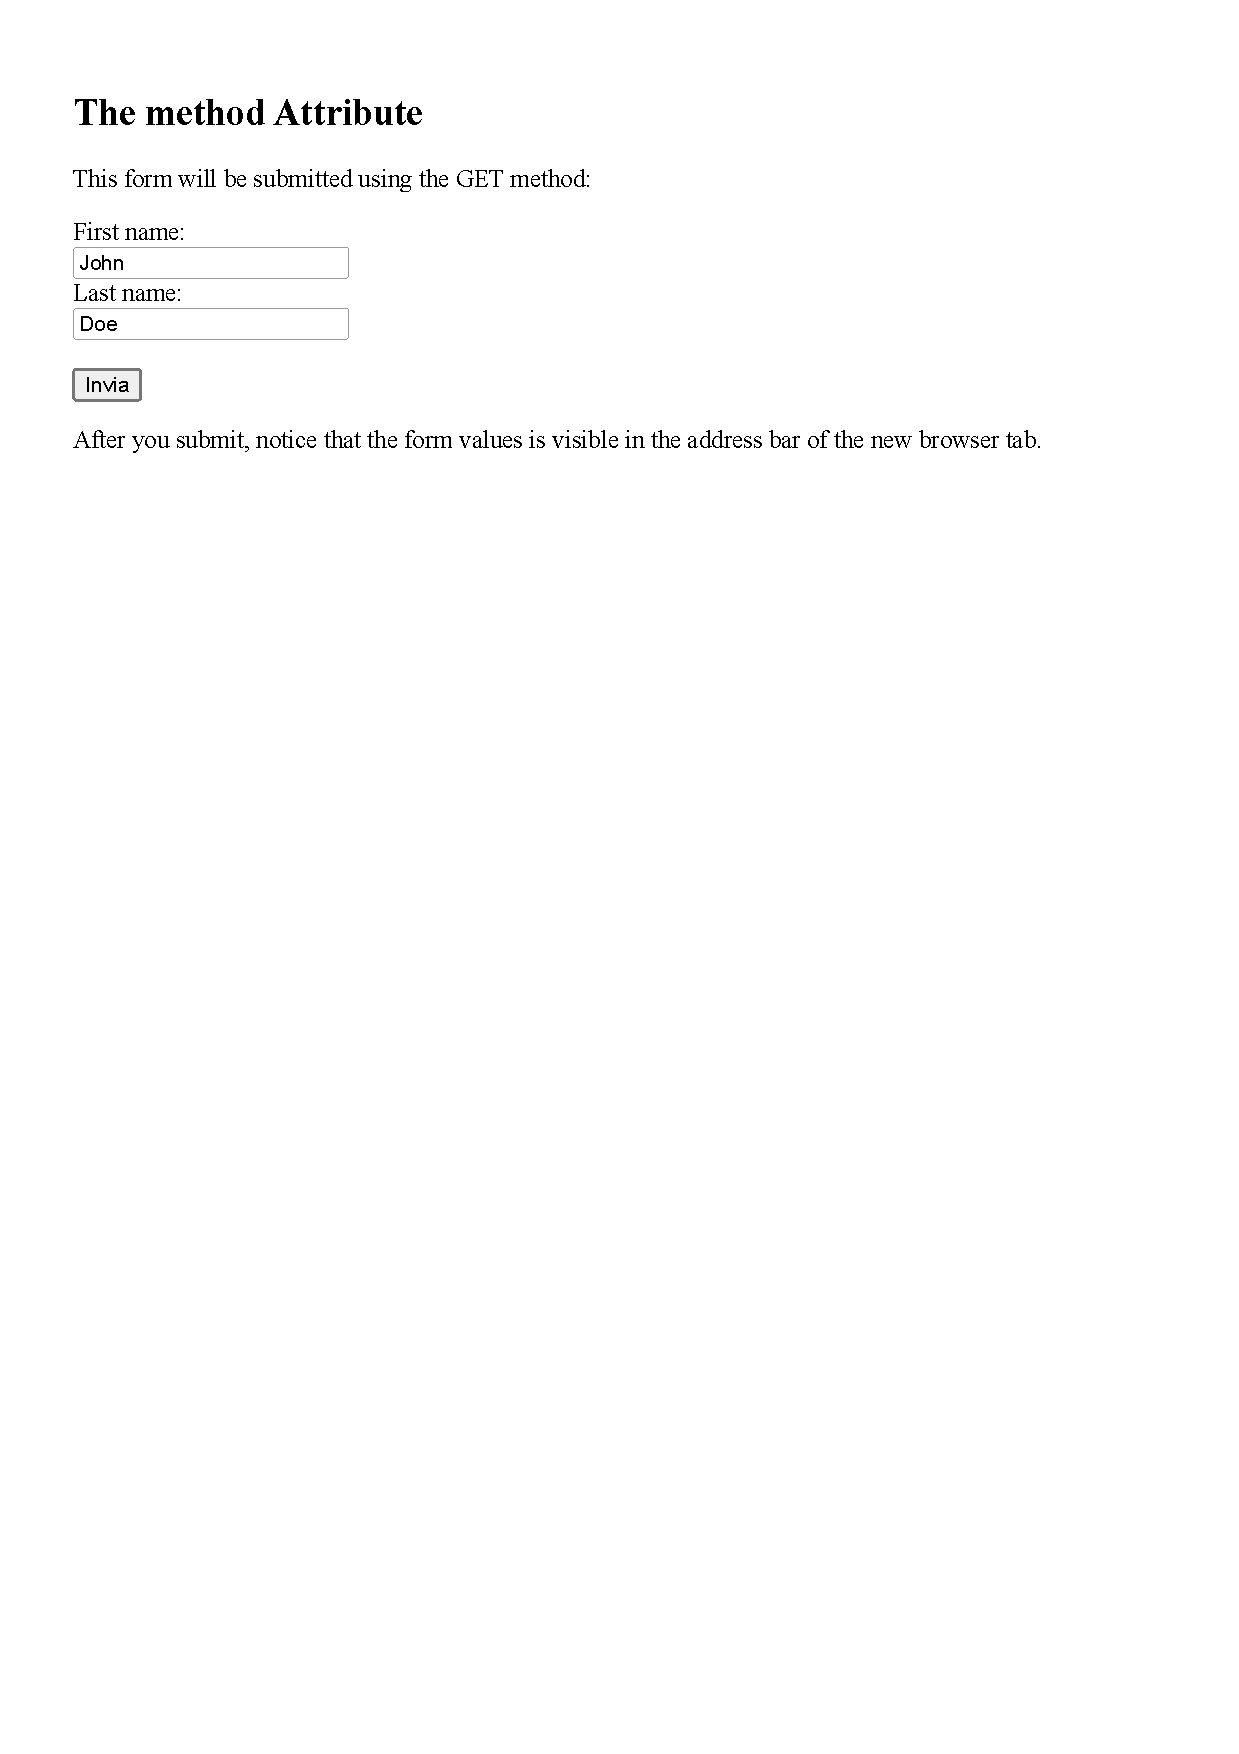
\includegraphics[width=\textwidth]{img/form-get.pdf}
	\end{figure}
	
	\noindent
	Una volta inserito nome e cognome, alla pressione del tasto, i dati saranno inviati al \emph{localhost} aggiungendo come parametri nell'URL \textsf{fname=name} e \textsf{lname=name}, dove al posto di name vengono inseriti nome e cognome. Il link risulta: \url{http://127.0.0.1/action?fname=John&lname=Doe}.\newpage
	
	\begin{figure}[!htp]
		\centering
		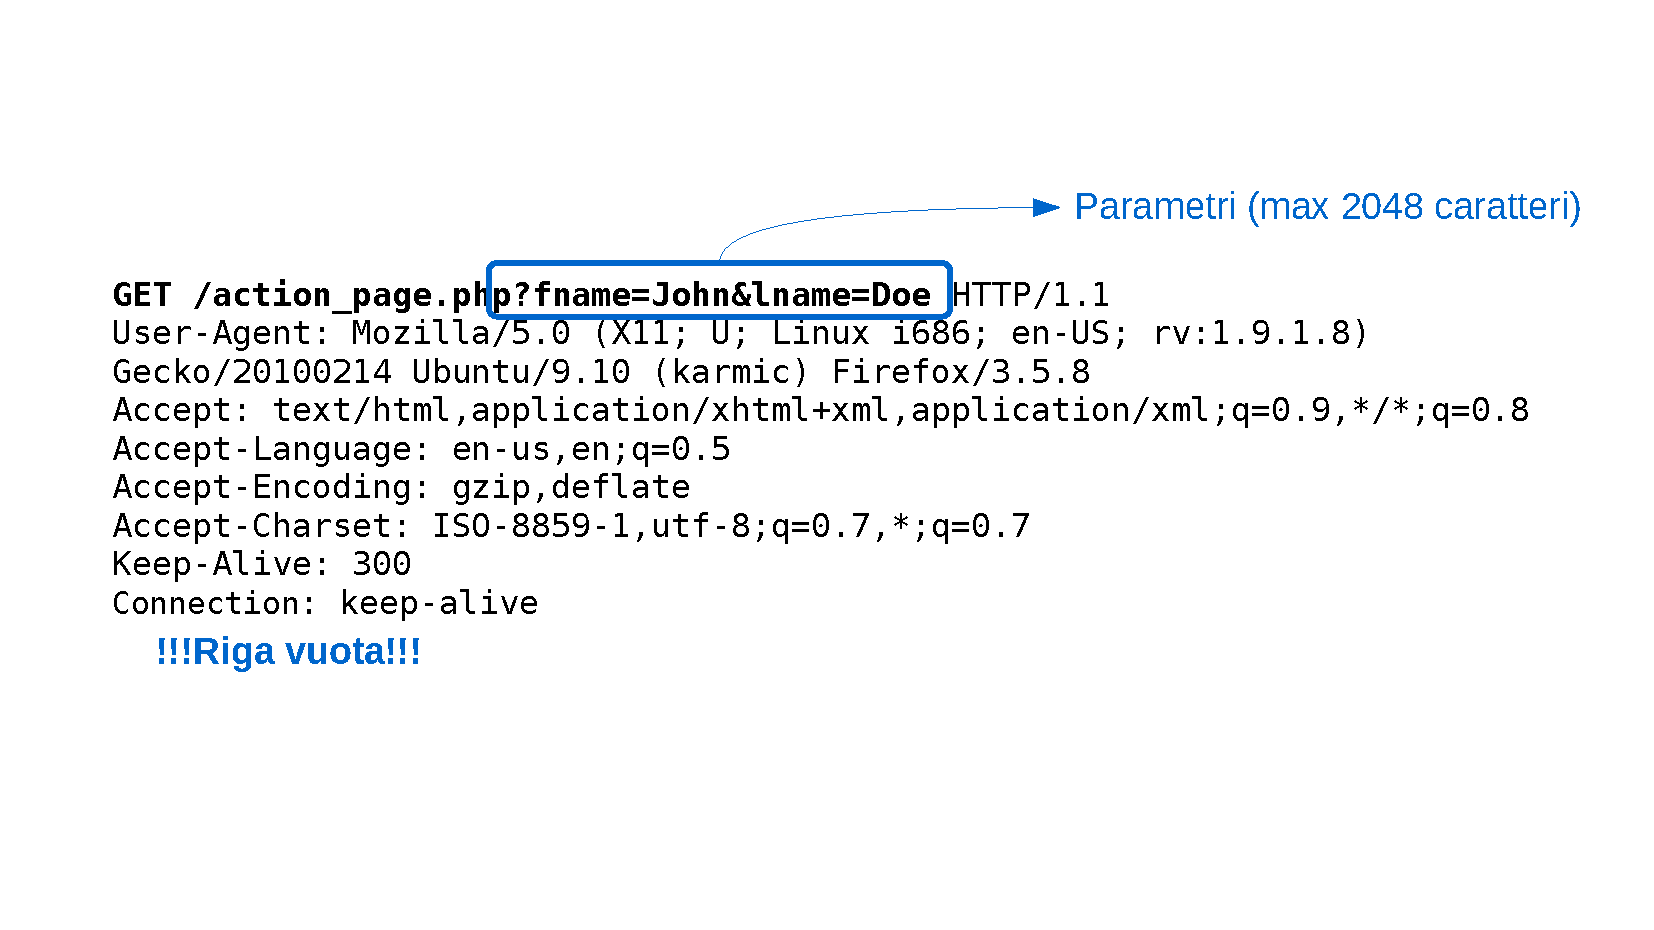
\includegraphics[width=\textwidth]{img/richiesta_get.pdf}
		\caption{La richiesta GET HTTP.}
	\end{figure}\newpage

	\subsection{Passare dei dati al server web col metodo POST}
	
	Il codice HTML per utilizzare il metodo POST è il seguente:
	\lstinputlisting[language=HTML]{code/form-post.html}
	La pagina web visualizzata è la seguente:
	\begin{figure}[!htp]
		\centering
		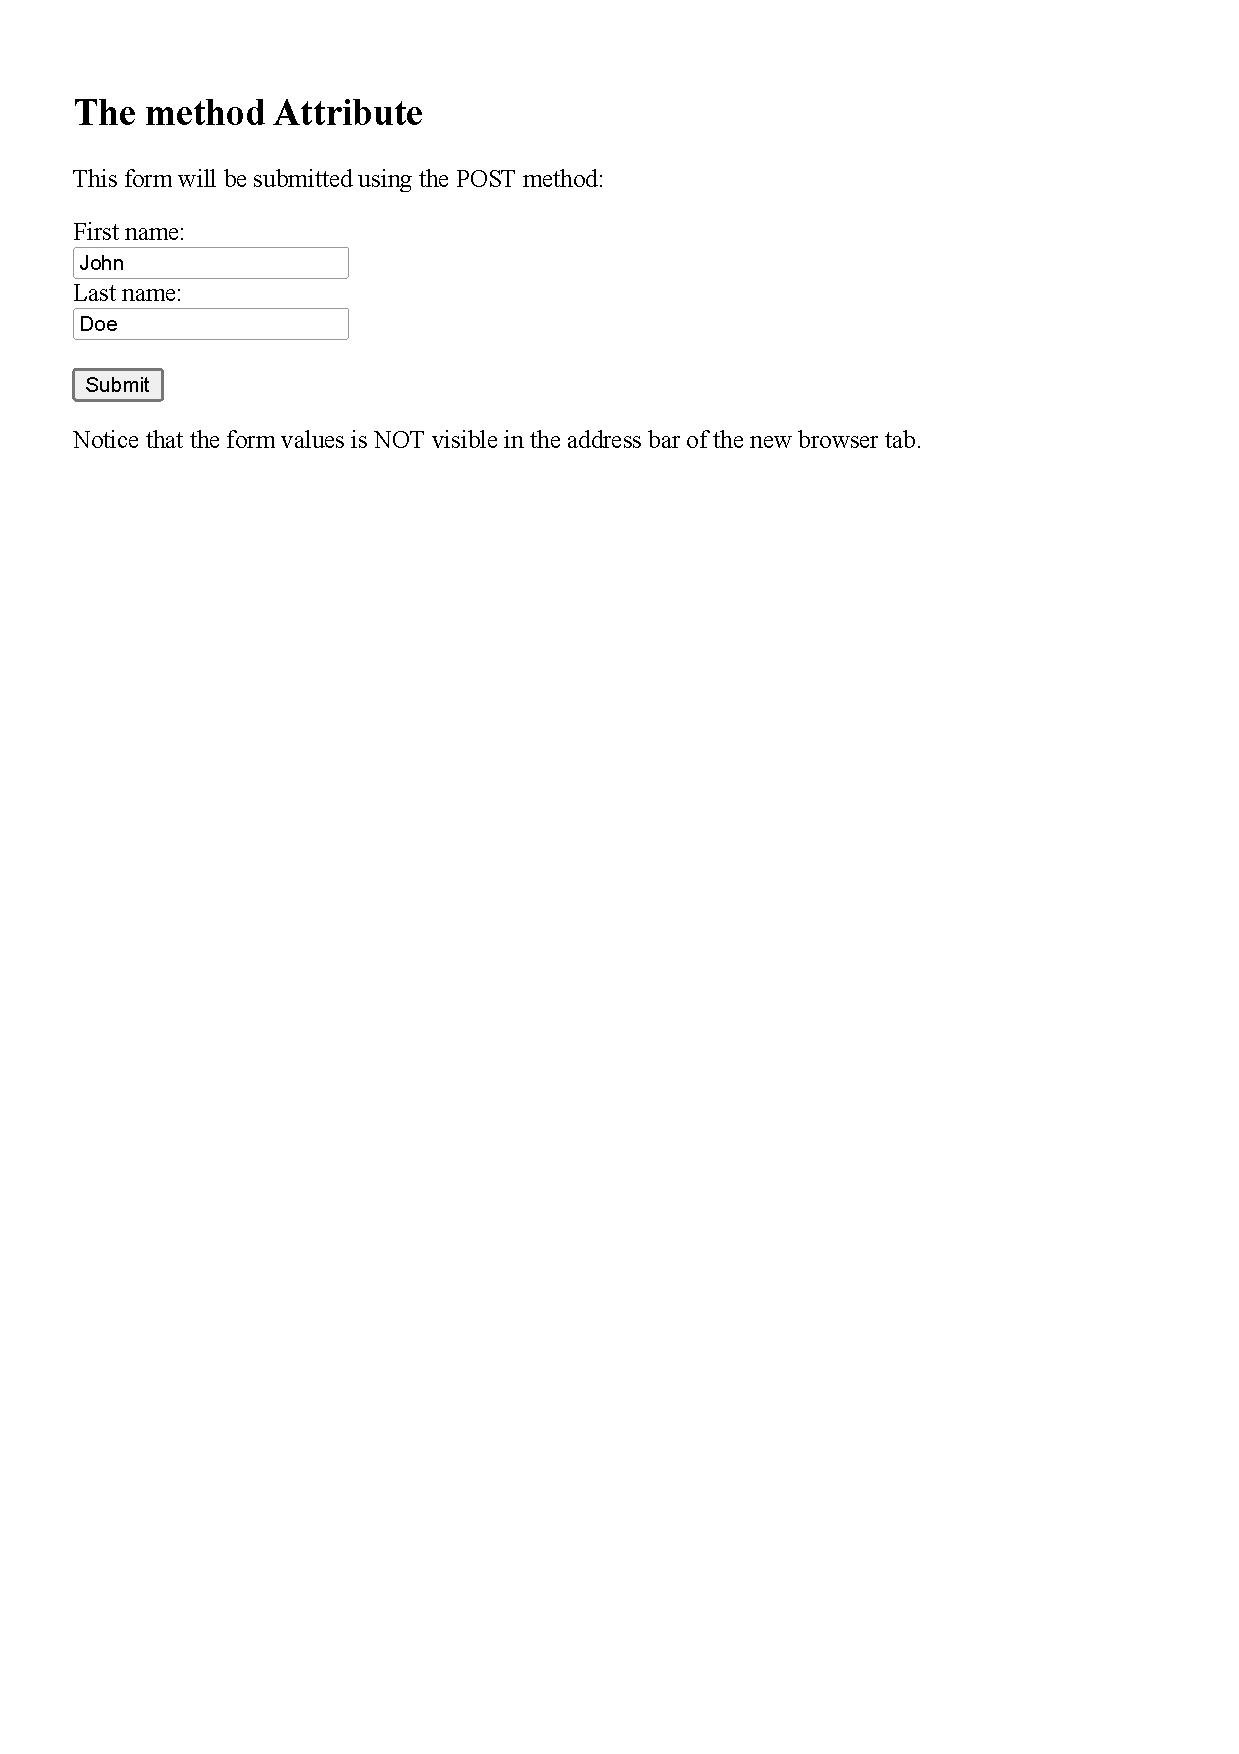
\includegraphics[width=\textwidth]{img/form-post.pdf}
	\end{figure}
	
	\noindent
	Una volta inserito nome e cognome, alla pressione del tasto, i dati saranno inviati al \emph{localhost}. \textbf{A differenza del metodo GET}, i parametri non vengono specificati nell'URL, di conseguenza la sicurezza aumenta. Il link dunque risulta: \url{http://127.0.0.1/action}.\newline
	
	\noindent
	I valori vengono inseriti all'interno della richiesta HTTP.\newpage
	
	\begin{figure}[!htp]
		\centering
		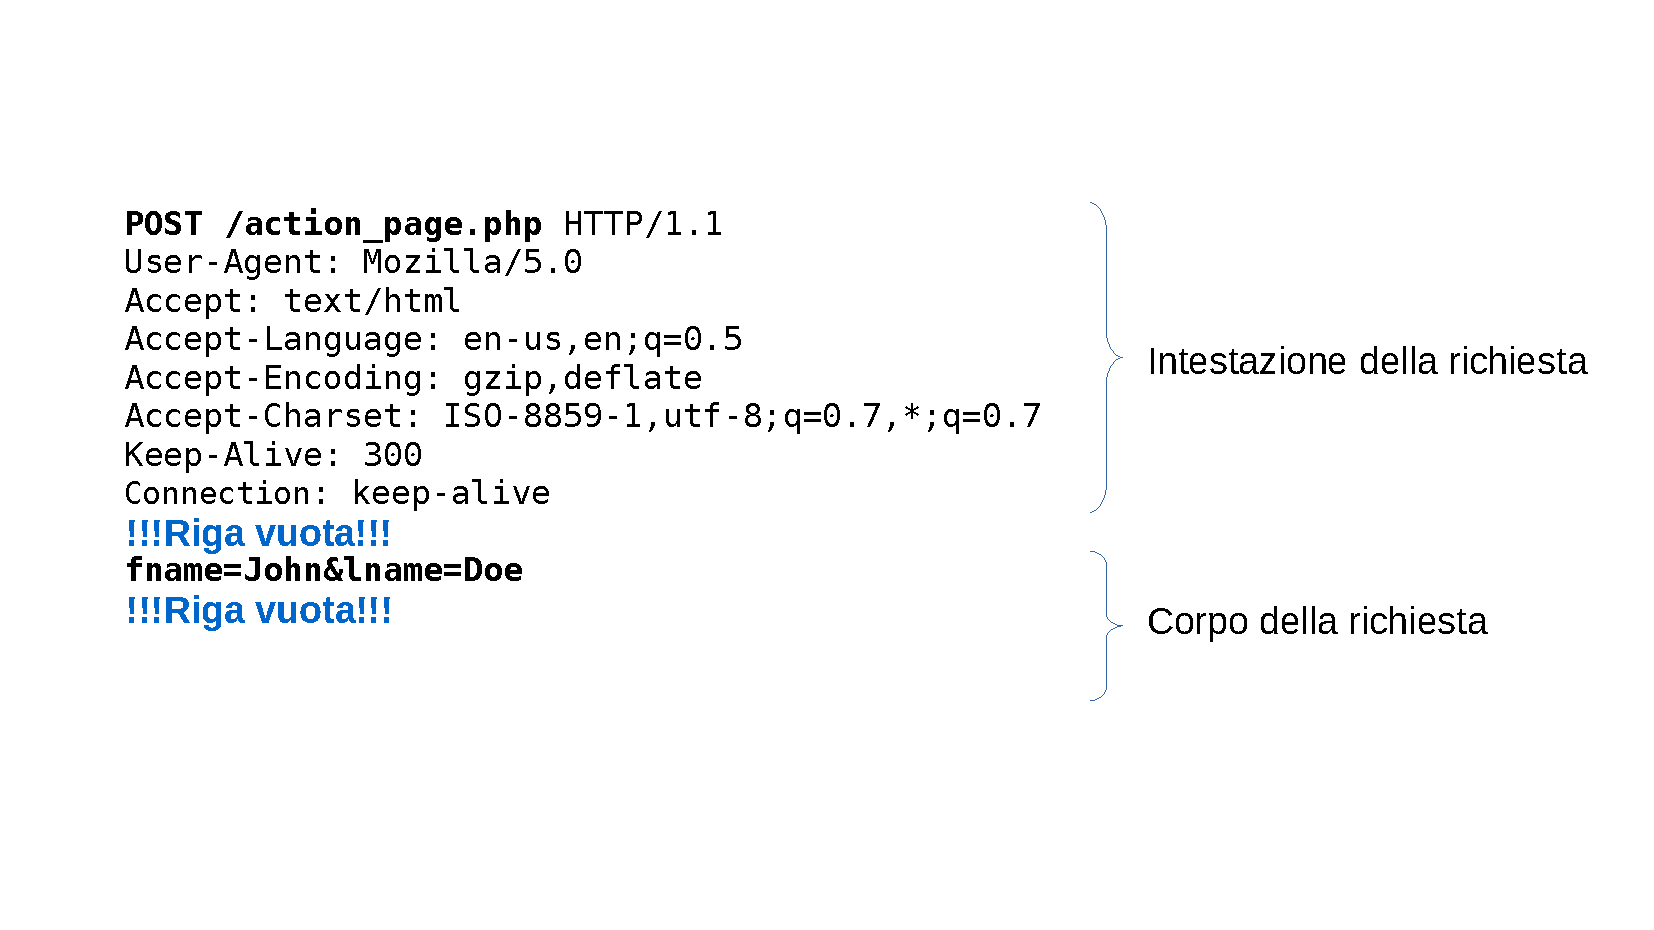
\includegraphics[width=\textwidth]{img/richiesta_post.pdf}
		\caption{La richiesta POST HTTP.}
	\end{figure}\newpage

	\subsection{Common Gateway Interface (CGI)}
	
	Il \textcolor{Red3}{\textbf{Common Gateway Interface (CGI)}} è una tecnologia utilizzata dai \emph{web server} per interfacciarsi con applicazioni esterne generando contenuti web dinamici.\newline
	
	\noindent
	Ogni qualvolta che un \emph{client} richiede al web server un URL corrispondente a un documento HTML, gi viene restituito un documento statico. Al contrario, se l'URL corrisponde a un programma CGI, il server lo esegue in tempo reale, generando dinamicamente informazioni per l'utente. Sostanzialmente è l'\textbf{esecuzione di un determinato programma sul server}.
	
	Di conseguenza, il browser diventa il \emph{client} di molte applicazioni di rete, per esempio la posta elettronica.
	
	\begin{figure}[!htp]
		\centering
		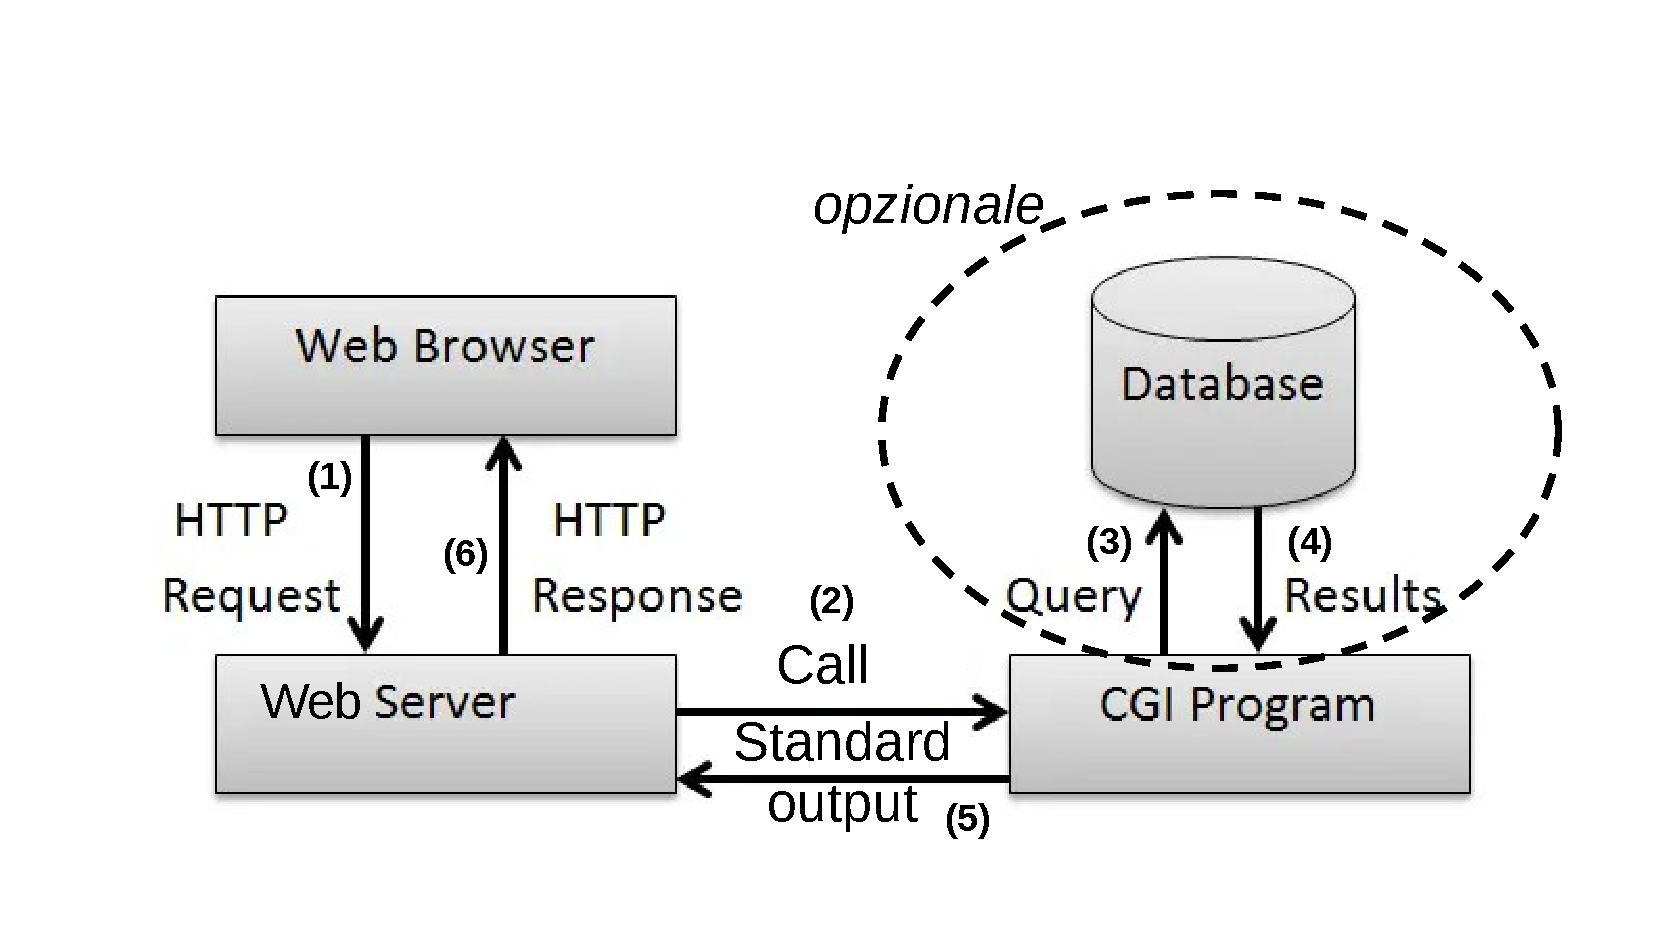
\includegraphics[width=\textwidth]{img/CGI.pdf}
		\caption{Fasi del CGI.}
	\end{figure}

	\noindent
	Degli \textcolor{Green4}{\textbf{esempi}} di esecuzione lato server di un programma sono un eseguibile come il client della posta elettronica, oppure un codice PHP, Java, NodeJS, ecc.\newpage
	
	\begin{figure}[!htp]
		\centering
		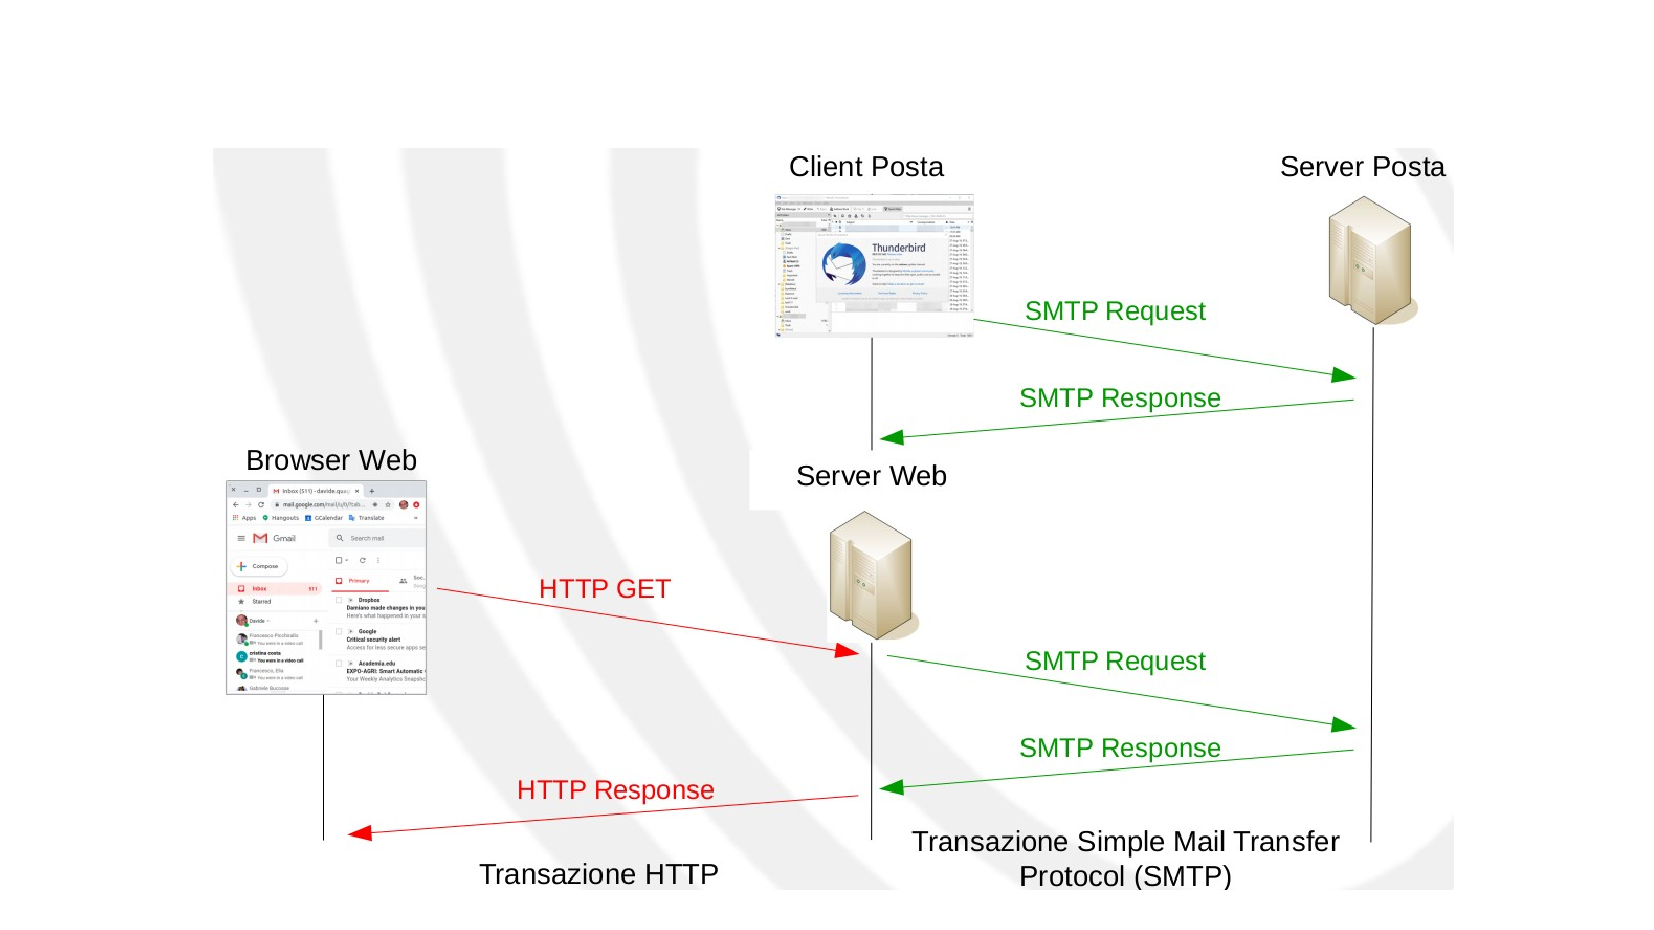
\includegraphics[width=\textwidth]{img/CGI_esempio.pdf}
		\caption{Esempio di CGI, la classica posta elettronica.}
	\end{figure}\newpage

	\subsection{Web socket}
	
	La \textcolor{Red3}{\textbf{web socket}} è una tecnologia web che fornisce canali di comunicazione chiamati \emph{full-duplex}, cioè bidirezionali, attraverso una singola connessione TCP. Viene utilizzato principalmente per realizzare applicazioni che forniscono contenuti e giochi in tempo reale. Questo perché \textbf{il protocollo consente maggiore interazione tra browser e server} grazie al alcune caratteristiche.\newline
	
	\noindent
	Innanzitutto è un \textbf{protocollo a livello di applicazione}, per cui è un \textbf{metodo alternativo a HTTP e HTTPS}. Ha la caratteristica fondamentale di \textbf{comunicazione simmetrica} tra \emph{browser} e \emph{web server}, ovverosia che \textbf{i processi possono \dquotes{prendere l'iniziativa} e inviare dei dati alla controparte}. Inoltre, nasce da una sessione HTTP/HTTPS attraverso un'operazione chiamata \textbf{Protocol Upgrade}.
	\begin{figure}[!htp]
		\centering
		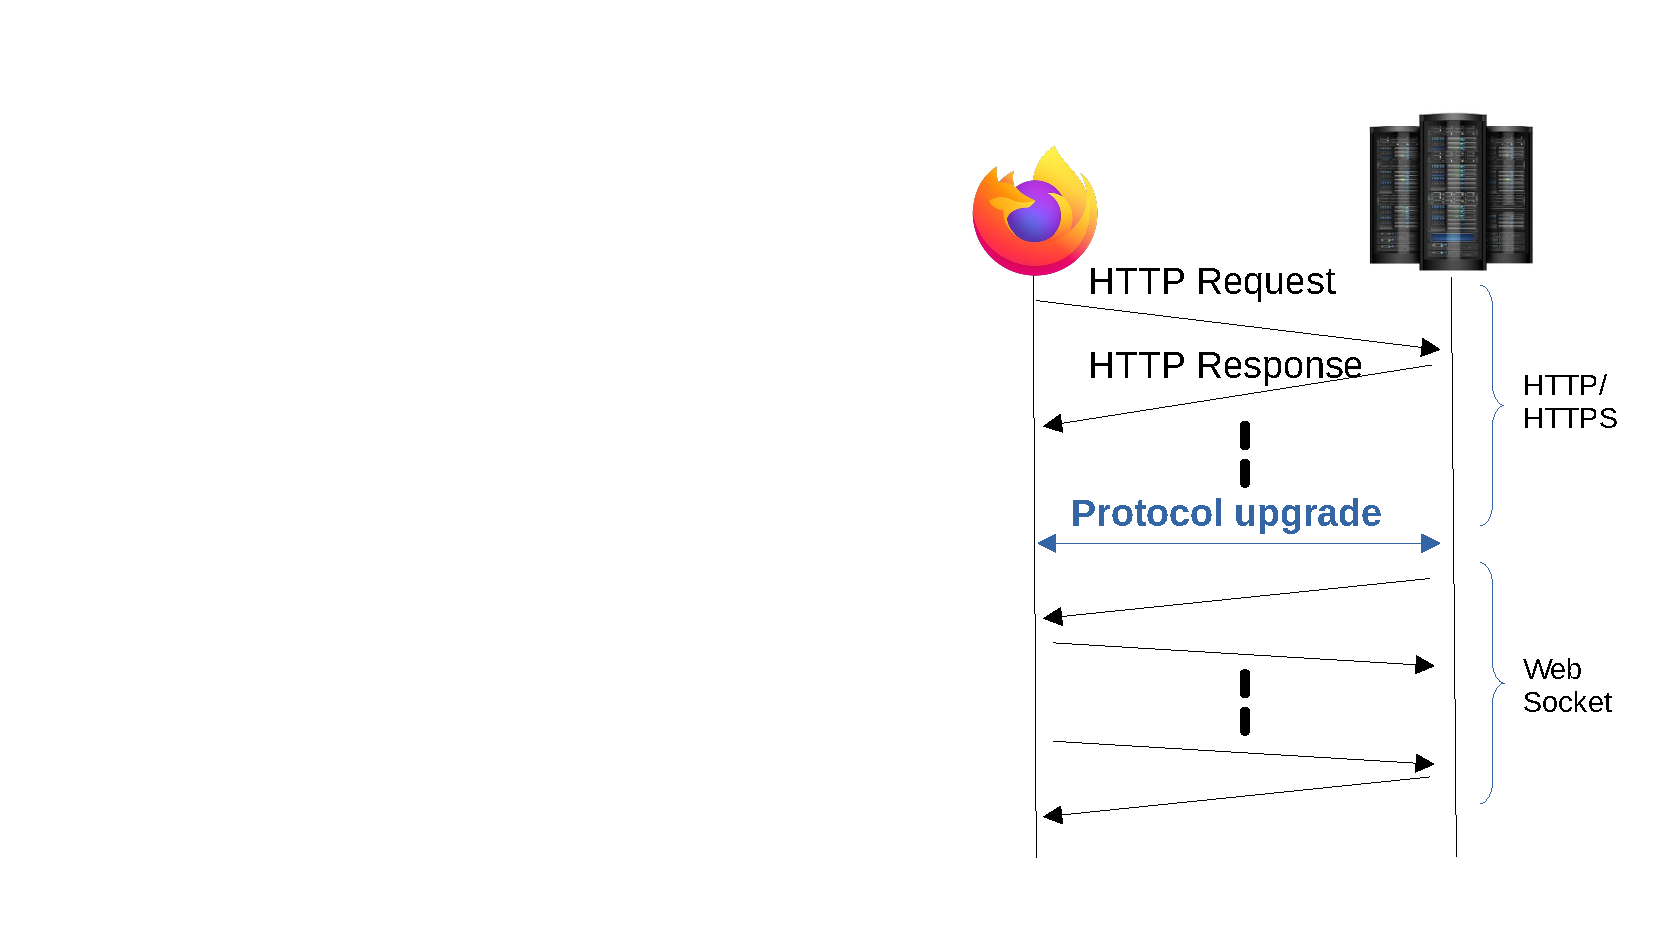
\includegraphics[width=.5\textwidth]{img/web_socket.pdf}
		\caption{Esempio di web socket e Protocol Upgrade.}
	\end{figure}
	
	\noindent
	Nel messaggio HTTP, ci sono due campi che vengono modificati per indicare il Protocol Upgrade: \textsf{Upgrade} e \textsf{Connection}. Entrambi i campi vengono modificati con i rispettivi valori \textsf{websocket} e \textsf{Upgrade}.\newpage
	
	\noindent
	\begin{figure}[!htp]
		\centering
		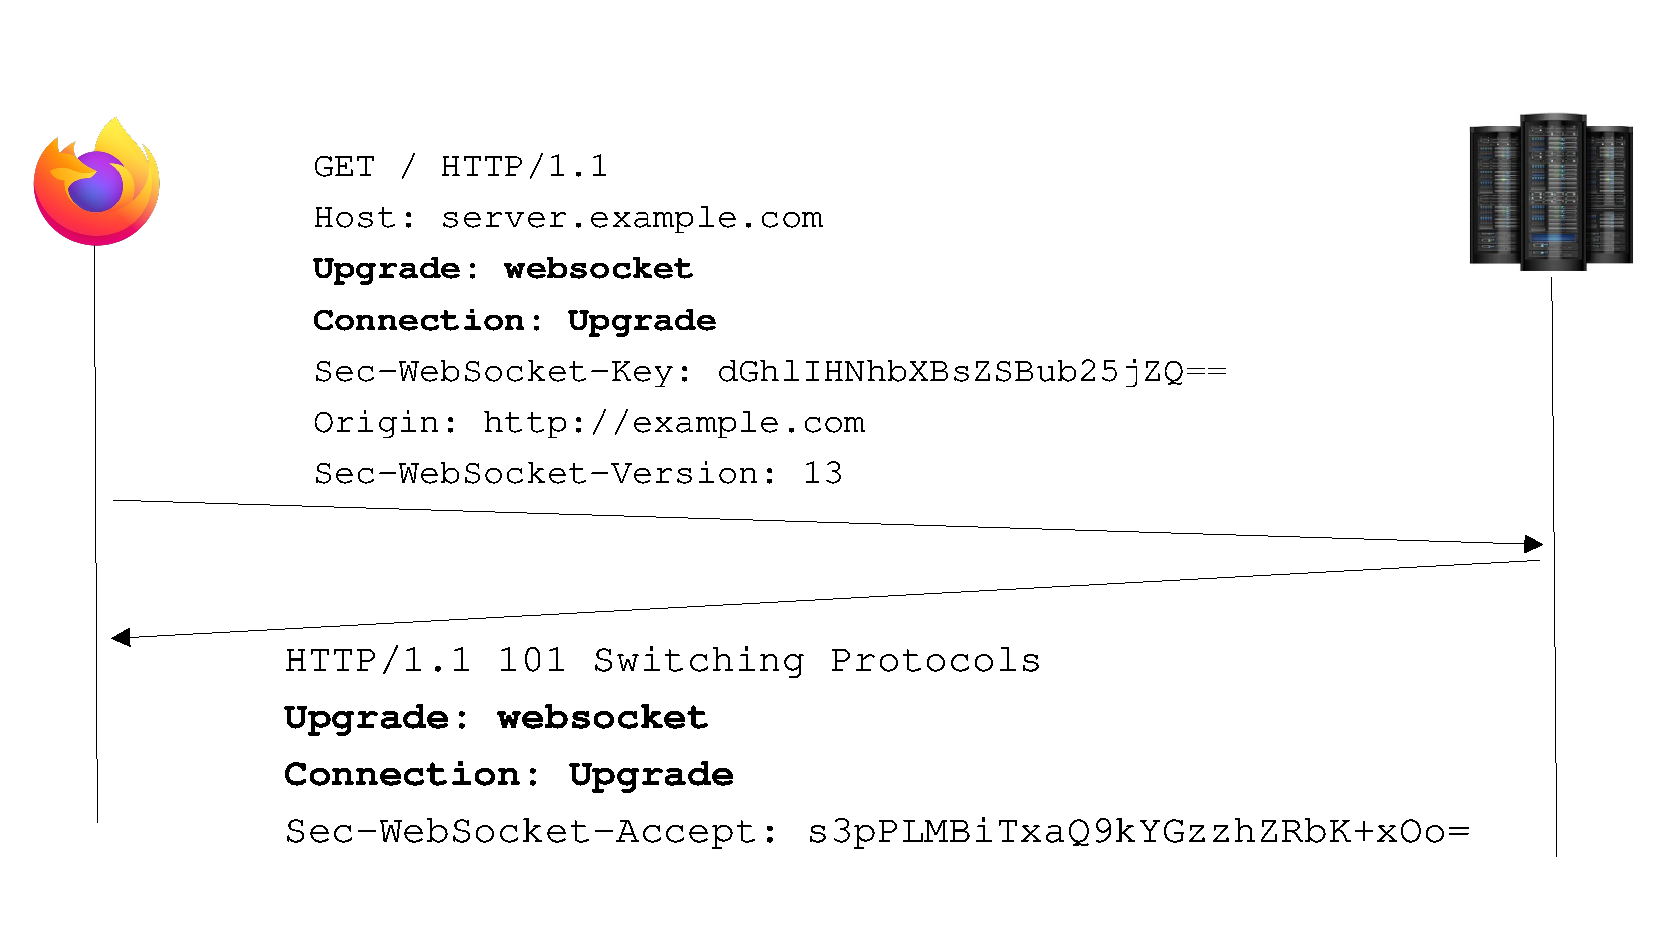
\includegraphics[width=\textwidth]{img/protocol_upgrade.pdf}
		\caption{Il Protocol Upgrade nel dettaglio.}
	\end{figure}
\end{document}